%-----------------Präambel-----------------%
\documentclass[a0,portrait]{a0poster}
\usepackage{multicol}
\usepackage[utf8]{inputenc}
\usepackage[T1]{fontenc}
\usepackage{ae}
\usepackage{lmodern}
\usepackage{helvet}
\renewcommand{\familydefault}{\sfdefault}
\newcommand{\changefont}[3]{\fontfamily{#1} \fontseries{#2} \fontshape{#3} \selectfont}
\usepackage[ngerman]{babel}
\usepackage{color}
\definecolor{darkgreen}{rgb}{0,0.5,0}
\definecolor{darkblue}{rgb}{0,0,0.5}
\definecolor{bluesky}{rgb}{0.63,0.80,1.0}
\usepackage{amsmath}
\usepackage{fancybox}
\usepackage{graphicx}
%-----------------Makros-----------------%
\renewcommand\baselinestretch{1.35}
\parskip=0.5\baselineskip
\parindent0mm %Einrücktiefe der ersten Zeile eines Absatzes
\topmargin-28pt
\marginparwidth0mm

%Ränder rechts/links
\oddsidemargin-13pt
\evensidemargin-13pt
\textwidth785mm
%\textheight1140mm

\newcommand{\spaltenbreite}{15}
\newcommand{\bildbreite}{15cm}

\setlength{\fboxrule}{3.25mm} 		%Definiert die Linienstärke für nachfolgende fbox- und framebox-Befehle
\setlength{\fboxsep}{5mm} 			%Abstand zwischen Rahmen und Text bei den /fbox und /framebox Befehlen.
\setlength{\columnsep}{15mm}     	%Spaltenabstand
\setlength{\columnseprule}{1pt}  	%Balken zwischen Spalten {0pt}->keine Balken

\unitlength1cm
\newcounter{skalax}
\newcounter{skalay}

% Literaturverzeichnis:
\usepackage[autostyle=true,german=quotes]{csquotes}
\usepackage[
backend=biber,
style=iso-numeric,
autolang=other,
bibencoding=UTF8,
maxnames=3,
hyperref
]{biblatex}

\DefineBibliographyStrings{ngerman}{andothers={et\ al\adddot}}
\addbibresource{Referenzen.bib}

\apptocmd{\UrlBreaks}{\do\f\do\m}{}{}
\setcounter{biburllcpenalty}{9000}% Kleinbuchstaben
\setcounter{biburlucpenalty}{9000}% Großbuchstaben

%-----------------Beginning-----------------%
\begin{document}

\begin{center}
	\vspace*{0.006\textheight}
	{\huge \textbf{Evaluierung von Methoden\\[-0.003\textheight]
			zur Bestimmung der ventilatorischen\\[-0.003\textheight]
			Schwellen in der Spiroergometrie}\\}%[0.03\textheight]
	\vspace*{0.018\textheight}
	{\LARGE \textbf{Julian-Marvin Lütten (2018)}}
\end{center}

\begin{picture}(0,0)
\put(66.5, 7){
\includegraphics[height=60mm]{Bilder/fhl_logo.eps}}
\put(66.4, 5.8){\textsf{\textbf{Prof. Dr. Dipl.-Ing. U. Wenkebach}}}
\put(0.0, 9.5){\includegraphics[height=33mm]{Bilder/cardioscan_logoclaim_RGB_pos.png}}
\end{picture}

\cornersize*{20mm}
\linethickness{0.1mm}
\setlength{\fboxrule}{2.25mm}

%%%%%%%%%%%%%%%%%%%%%%%%%%%%%%%%%%%%%%%%%%%%%%%%%%%%%%%%%%%%%%%%%%%%%%% 
% neuer Kasten
\Ovalbox
{
	\parbox{\textwidth}{
		\begin{multicols}{3}
			\begin{center} \textbf{\Large Einleitung} \end{center}
Die Spiroergometrie (aus lat. \textsl{spirare}: atmen, griech. \textsl{ergo}: Arbeit) ist eine oft genutzte technische Anwendung der Sportmedizin zur Bestimmung von individuellen Trainingsbereichen, bei der respiratorische Daten während inkrementierter körperlicher Belastung erfasst und anschließend analysiert werden. Der Hamburger Medizintechnik-Hersteller cardioscan GmbH hat 2017 ein Spiroergometer entwickelt, welches in Verbindung mit einer Software für dieses Verfahren noch nicht getestet wurde. Die Software verwendet momentan einen Algorithmus, der recht sensitiv für Fehler ist und deshalb durch einen neuen ersetzt werden muss. Hierfür eignen sich Methoden zur Bestimmung der Ventilatorischen Schwellen VT1 und VT2, die von der AG Spiroergometrie empfohlen werden~\cite{Westhoff.2012}.\\
Es wurden im Rahmen dieser Arbeit insgesamt vier Methoden ausgewählt, die in Folge an eine Spiroergometrie mit dem neuen Gerät des Unternehmens bestimmt werden sollten. Zu überprüfen war, ob das Gerät generell für diese Anwendung nutzbar ist, welche der vier Methoden zum Erreichen der Firmenziele optimal ist und ob die Methoden genauere Ergebnisse liefern können, als der ursprüngliche Algorithmus.





			\textbf{\Large Grundlagen}\\

Das ventilatorische Schwellenkonzept basiert auf der physiologischen Reaktion des Körpers auf die zunehmende Belastung bei einer Spiroergometrie. Da der Muskelgehalt des körpereigenen Energiestoffs ATP zur Muskelkontraktion nur für eine kurze Zeit ausreicht, muss dieser für andauernde Arbeit durch Glykolyse resynthetisiert werden \cite{Kroidl.2015}. Reicht ab einer bestimmten Belastung die Sauerstoffaufnahme (\.{V}O\textsubscript{2}) nicht mehr aus, funktionieren gewisse, für die Glykolyse notwendige Coenzyme nicht mehr, sodass in den Muskeln Laktat akkumuliert und es allmählich zur metabolischen Azidose (Übersäuerung) kommt. Der Körper kompensiert dies durch Puffer-Reaktionen, wodurch überschüssiges Kohlenstoffdioxid (CO\textsubscript{2}) anfällt, welches abgeatmet wird und respiratorisch gemessen werden kann.\\
Nach einer Spiroergometrie werden Atemparameter grafisch verglichen, um ventilatorische Reaktionen auf biochemische Prozesse zu detektieren. Die ventilatorischen Schwellen stellen Stoffwechselübergänge dar, anhand derer mit verschiedenen Modellen Trainingsbereiche bestimmbar sind. Sie werden für üblich als Herzfrequenz in \si{\per\minute} angegeben. Die VT1 wird mittels der V-Slope-Methode oder anhand des Sauerstoff-Äquivalents (EQO\textsubscript{2}) grafisch identifiziert. Das Kohlenstoffdioxid-Äquivalent (EQCO\textsubscript{2}) oder der Vergleich der Ventilation (\.{V}E) zur Kohlenstoffdioxidabgabe (\.{V}CO\textsubscript{2}) eignen sich zur Bestimmung der VT2.\\

\begin{picture}(\spaltenbreite,6)
\put(0.9,2){\includegraphics[width=50mm]{Bilder/vslope.png}}
\put(1.6,0.7){\parbox{720pt}{{\bf \small a):} \small V-Slope}}
\put(7.1,2){\includegraphics[width=50mm]{Bilder/eqo2.png}}
\put(8.1,0.7){\parbox{720pt}{{\bf \small b)} \small EQO\textsubscript{2}}}
\put(13.3,2){\includegraphics[width=50mm]{Bilder/eqco2.png}}
\put(14.1,0.7){\parbox{720pt}{{\bf \small c)} \small EQCO\textsubscript{2}}}
\put(19.6,2){\includegraphics[width=50mm]{Bilder/field4.png}}
\put(20.1,0.78){\parbox{720pt}{{\bf \small d)} \small \.{V}E/\.{V}CO\textsubscript{2}}}
\put(1.4,-0.6){\parbox{720pt}{{\bf \small Abb. 1:} \small Methoden zur Schwellenbestimmung: VT1: blau; VT2: orange}}
\end{picture}

		\end{multicols}
	}
}

% neuer Kasten
\vspace*{0.002\textheight}
\Ovalbox%\fbox
{
	\parbox{\textwidth}{
		\begin{multicols}{3}
			\begin{center} \textbf{\Large Methode} \end{center}

In einem firmeninternen Projekt wurden mit 28 unterschiedlichen Probanden nach einem gleichen festgelegten Prozedere spiroergometrische Tests auf einem Fahrradergometer durchgeführt, bei der die Herzfrequenz zusätzlich über einen Pulsgurt erfasst wurde. Die Sensor-Rohdaten des Spiroergometers, die Herzfrequenz sowie die Leistungswerte des Ergometers wurden durch ein MATLAB-Programm weiterverarbeitet und grafisch in Form von eigens erstellten "`6-Felder-Grafiken"' visualisiert. In diesen sind die Plots für alle vier Methoden enthalten. Die Grafiken wurden subjektiv von zwei Ratern sowie mathematisch durch einen Algorithmus analysiert. Anschließend wurden die Ergebnisse der unterschiedlichen Methoden statistisch miteinander verglichen und Differenzen bzw. Abweichungen bei den identifizierten Schwellen untersucht. Die Ergebnisse wurden außerdem mit den Erkenntnissen der HUNT 3 Studie aus dem Jahre 2014 verglichen, um zu diskutieren, ob die individuell gemessenen Werte realistisch waren.

			\textbf{\Large Resultate}
\vspace*{1.6em}\\
Bei den Testmessungen traten keinerlei Gerätefehler oder Störungen auf, sodass für alle 28 Probanden Ergebnisse in Form von Graphen erstellt werden konnten. Abb. 5 zeigt ein Beispiel einer 6-Felder-Grafik, in der die respiratorischen Parameter in verschiedenen Farben aufgetragen sind. Zum Ablesen der ventilatorischen Schwellen ist die entsprechend gemessene Herzfrequenz in Form einer rosafarbenen Linie in die Plots integriert.

\begin{center}
\begin{picture}(\spaltenbreite,16)
\put(-2.5,3){\includegraphics[width=200mm]{Bilder/plot_6w.jpg}}
\put(1.3,1.5){\parbox{720pt}{{\bf \small Abb. 5:} \small Beispiel einer 6-Felder-Grafik}}
\end{picture}
\end{center}


			\begin{center}
\begin{picture}(\spaltenbreite,20)
\put(-4,10){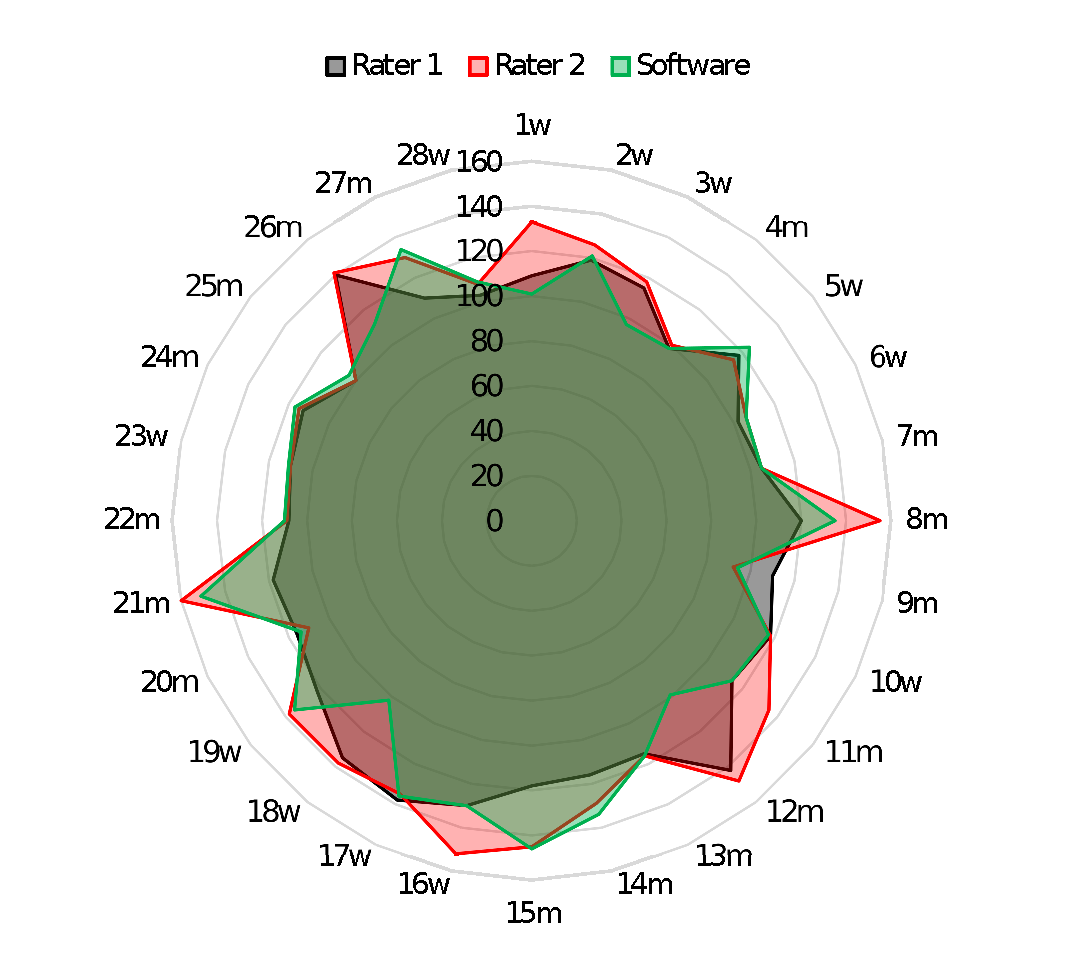
\includegraphics[width=110mm]{Bilder/v-slope_net.eps}}
\put(-2.9,9){\parbox{720pt}{{\bf \small Abb. 6:} \small V-Slope-Streuung}}
\put(8,10){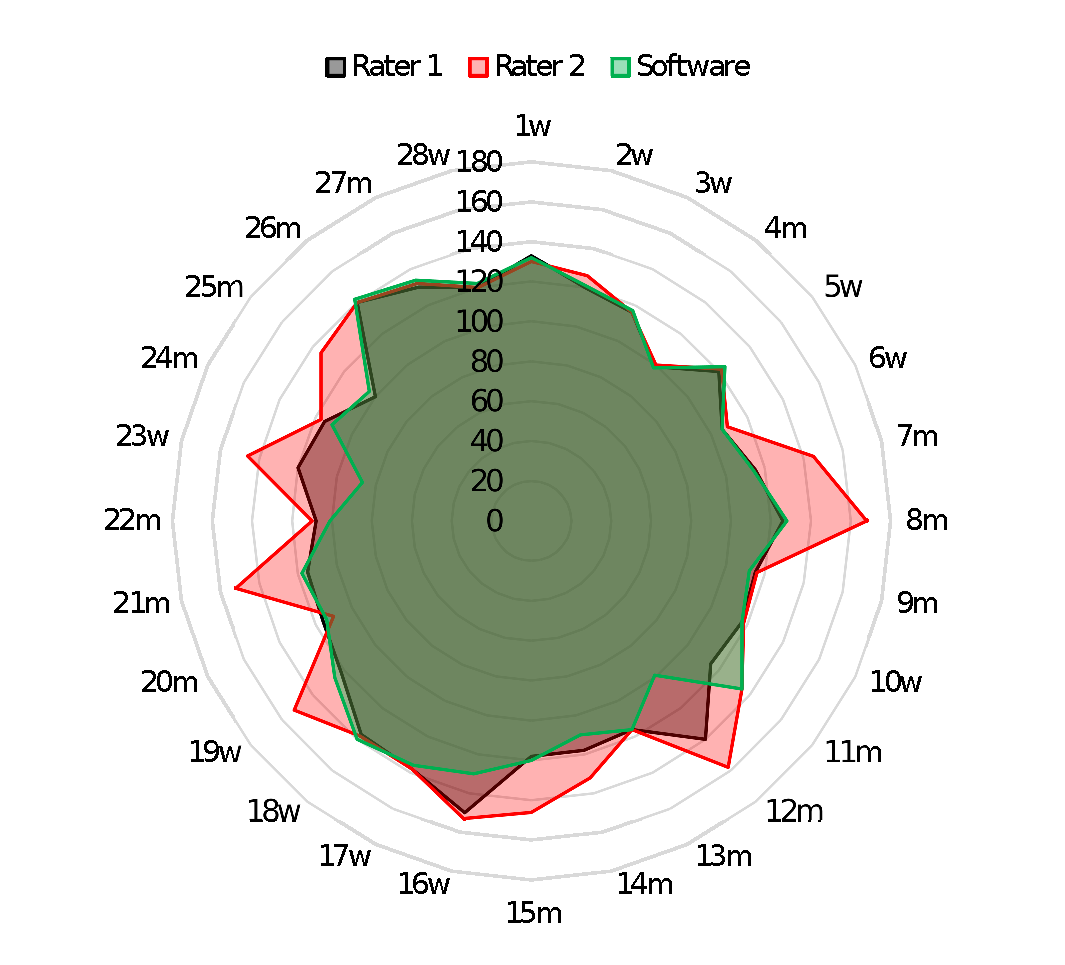
\includegraphics[width=110mm]{Bilder/eqo2_net.eps}}
\put(9.4,9){\parbox{720pt}{{\bf \small Abb. 6:} \small EQO\textsubscript{2}-Streuung}}
\put(-4,-3){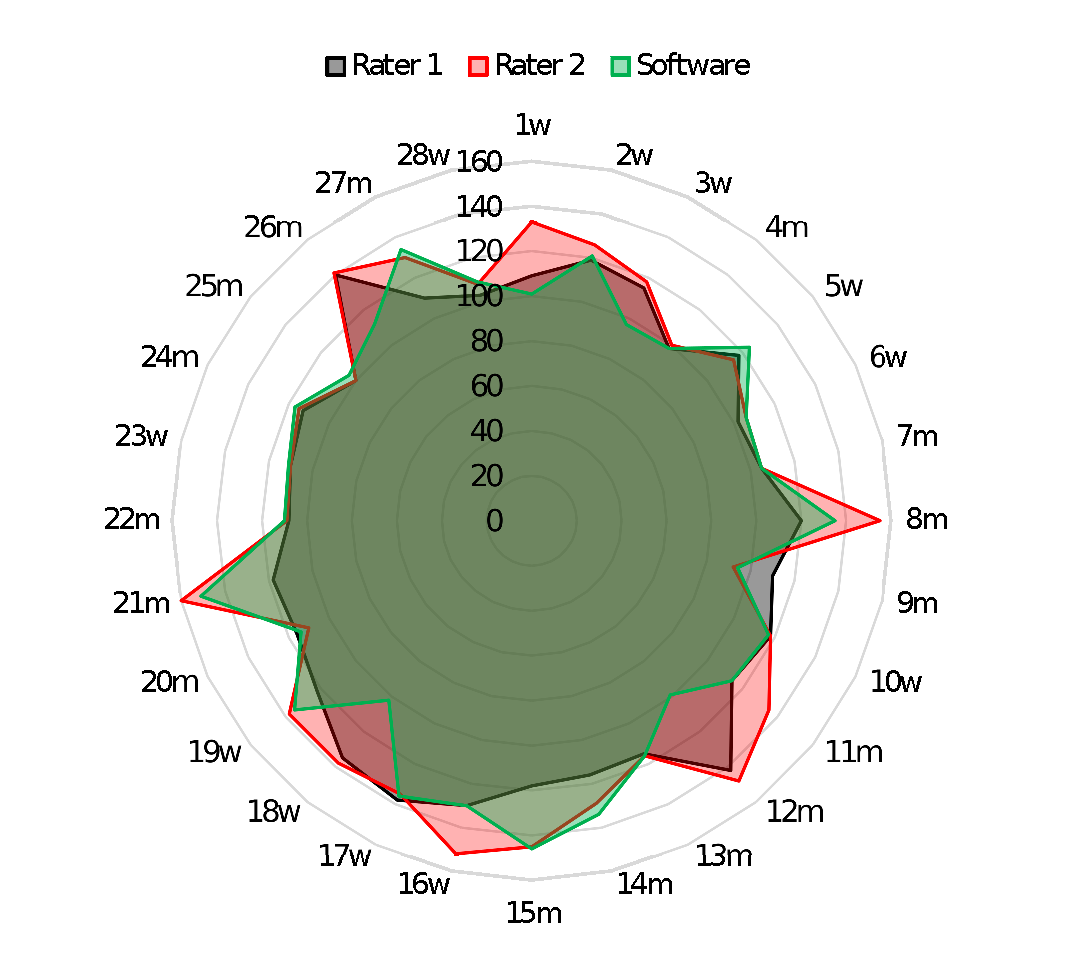
\includegraphics[width=110mm]{Bilder/v-slope_net.eps}}
\end{picture}
\end{center}
		\end{multicols}
	}
}

\end{document}